\subsection{SM4默认循环与循环展开} %默认循环和循环展开

\subsubsection{SM4默认循环}
按照课本介绍SM4算法的实现,不采用任何优化策略,完整实现SM4的32轮迭代并在每一轮计算中对明文分组做非线性变换S和线性变换L,记录
算法运行时间,并以此组作为基准组,
时间开销主要在32轮迭代以及每轮迭代中的S和L操作:
\begin{lstlisting}[title={openhitls/testcode/demo/sm4\_default\_loop.c}]
static void sm4EncryptBlock(const uint32_t rk[32],
                            const uint8_t in[16],
                            uint8_t out[16])
{
    uint32_t X[4];
    sm4LoadBlock(in, X);

    for (int i = 0; i < 32; i++) {
        uint32_t tmp   = X[1] ^ X[2] ^ X[3] ^ rk[i];
        uint32_t t     = sm4T(tmp);
        uint32_t newX0 = X[0] ^ t;
        X[0] = X[1];
        X[1] = X[2];
        X[2] = X[3];
        X[3] = newX0;
    }

    sm4StoreBlock(X, out);
}
\end{lstlisting}

结果如下:
\begin{figure}[H]
    \centering
    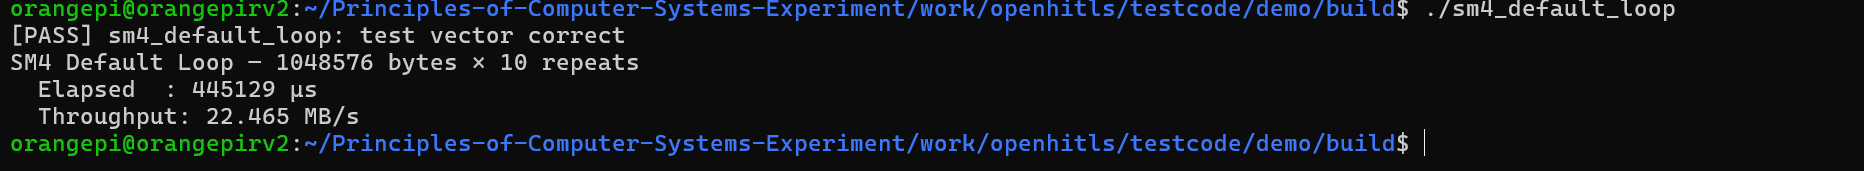
\includegraphics[width = 1\textwidth]{figure/sm4_default_loop.png}
\end{figure}
其中测试输入数据大小为1MB。

\subsubsection{SM4循环展开}
上述的循环次数以及每次循环的操作是已知的,使用宏一次性生成全部32轮代码,可以去掉32次i++和条件判断,避免分支预测失败惩罚,
同时再使用数组而是四个变量即可实现32轮循环迭代,省去计算数组索引和基于偏移量取数的开销,关键代码如下:
\begin{lstlisting}[title={openhitls/testcode/demo/sm4\_unrolled.c}]
static void sm4EncryptBlock(const uint32_t rk[32],
                            const uint8_t in[16],
                            uint8_t out[16])
{
    uint32_t X0, X1, X2, X3;
    uint32_t tmp, t, newX;

    /* Manual load to scalars for unrolled access */
    {
        uint32_t arr[4];
        sm4LoadBlock(in, arr);
        X0 = arr[0]; X1 = arr[1]; X2 = arr[2]; X3 = arr[3];
    }

#define SM4_UNROLLED_ROUND(N) do {         \
    tmp  = X1 ^ X2 ^ X3 ^ rk[N];           \
    t    = sm4T(tmp);                      \
    newX = X0 ^ t;                         \
    X0 = X1; X1 = X2; X2 = X3; X3 = newX;  \
} while(0)

    SM4_UNROLLED_ROUND(0);
    SM4_UNROLLED_ROUND(1);
    SM4_UNROLLED_ROUND(2);
    SM4_UNROLLED_ROUND(3);
    SM4_UNROLLED_ROUND(4);
    SM4_UNROLLED_ROUND(5);
    SM4_UNROLLED_ROUND(6);
    SM4_UNROLLED_ROUND(7);
    SM4_UNROLLED_ROUND(8);
    SM4_UNROLLED_ROUND(9);
    SM4_UNROLLED_ROUND(10);
    SM4_UNROLLED_ROUND(11);
    SM4_UNROLLED_ROUND(12);
    SM4_UNROLLED_ROUND(13);
    SM4_UNROLLED_ROUND(14);
    SM4_UNROLLED_ROUND(15);
    SM4_UNROLLED_ROUND(16);
    SM4_UNROLLED_ROUND(17);
    SM4_UNROLLED_ROUND(18);
    SM4_UNROLLED_ROUND(19);
    SM4_UNROLLED_ROUND(20);
    SM4_UNROLLED_ROUND(21);
    SM4_UNROLLED_ROUND(22);
    SM4_UNROLLED_ROUND(23);
    SM4_UNROLLED_ROUND(24);
    SM4_UNROLLED_ROUND(25);
    SM4_UNROLLED_ROUND(26);
    SM4_UNROLLED_ROUND(27);
    SM4_UNROLLED_ROUND(28);
    SM4_UNROLLED_ROUND(29);
    SM4_UNROLLED_ROUND(30);
    SM4_UNROLLED_ROUND(31);

#undef SM4_UNROLLED_ROUND

    /* Reverse transform & store */
    {
        uint32_t arr[4] = {X0, X1, X2, X3};
        sm4StoreBlock(arr, out);
    }
}
\end{lstlisting}
这里所有宏会在编译阶段就计算出来,能降低运行时计算的时间开销。运行结果如下:
\begin{figure}[H]
    \centering
    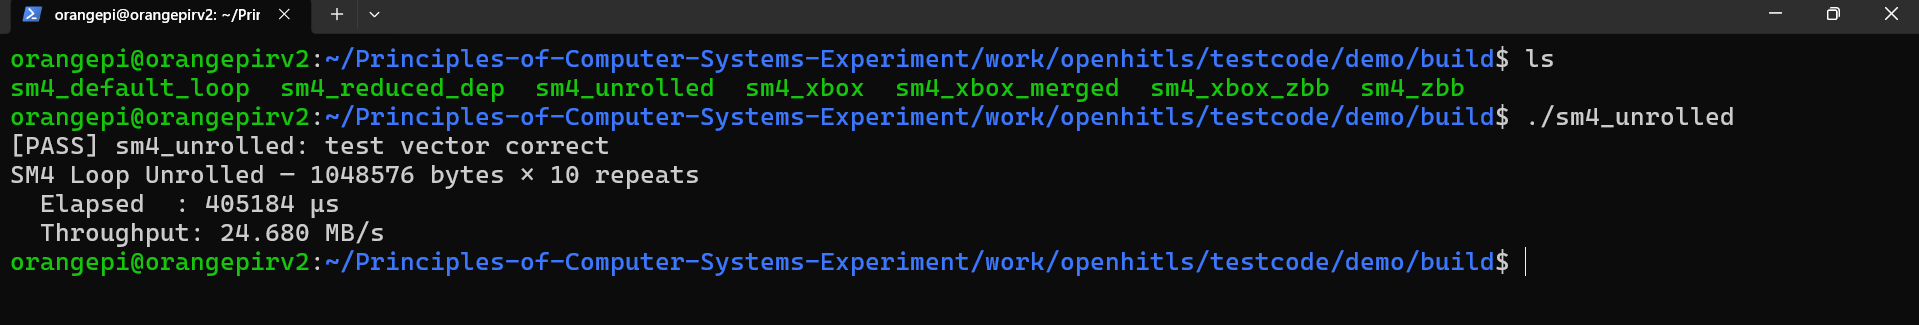
\includegraphics[width = 1\textwidth]{figure/sm4_unroll.png}
    \caption{SM4循环展开}
\end{figure}
可以看到循环展开能有效提升SM4加密算法的运行效率,提升吞吐量。